\documentclass[a4paper,11pt]{article}
\usepackage[osf]{mathpazo}
\usepackage{ms}
\usepackage{natbib}
\usepackage{graphicx}
\usepackage{caption}
\usepackage{hyperref}
\usepackage[labelfont=bf]{caption} % make label for figure bold

% Allow referencing into the supporting information, once that exists.
\IfFileExists{./competition-kernels-sm.tex}{%
  \usepackage{xr}%
  \externaldocument{competition-kernels-sm}}{}

% We will generate all images so they have a width \maxwidth. This means
% that they will get their normal width if they fit onto the page, but
% are scaled down if they would overflow the MAPgins.
\makeatletter
\def\maxwidth{\ifdim\Gin@nat@width>\linewidth\linewidth\else\Gin@nat@width\fi}
\def\maxheight{\ifdim\Gin@nat@height>\textheight\textheight\else\Gin@nat@height\fi}
\makeatother
\setkeys{Gin}{width=\maxwidth,height=\maxheight,keepaspectratio}

\title{Trait gradients}

\author{ Georges Kunstler, Daniel S. Falster, Richard G. FitzJohn}
\date{}
\affiliation{Department of Biological Sciences, Macquarie University,
  Sydney, Australia}
\runninghead{}
\keywords{}

\usepackage{color}

\newcommand{\ud}{\ensuremath{\mathrm{d}}}
\newcommand{\sign}{\mathop{\mathrm{sign}}\nolimits}
\newcommand{\Rstar}{\ensuremath{R^*}}
\newcommand{\plant}{{\tt plant}}
\newcommand{\hmat}{\ensuremath{h_{\text{mat}}}}
\newcommand{\TODO}{{\color{red}\sc todo}}


\begin{document}

\mstitleshort
%\mstitlepage
\parindent=1.5em
\addtolength{\parskip}{.3em}

% \begin{abstract}
% Abstract goes here\ldots
% \end{abstract}

\section{Background \& Motivation}

Understanding changes in vegetation composition across large biogeographic gradients is fundamental because vegetation is key to control ecosystem functioning, such as net primary production, and carbon storage. These changes in composition are also fundamental to understand biodiversity, as turnover in species composition explain a large proportion of the global diversity ($\beta$ diversity). In addition, these patterns are also the outcomes of long-term evolutionary adaptation. Understanding the drivers of these patterns is important not only for its intrinsic interest, but also as a path towards understanding how vegetation may change as result of environmental change.

Beyond species succession pattern along climatic gradients, several studies document gradient of key leaf and stem traits with precipitation (see literature.pdf for a in progress review of the literature), with consistent patterns of decreasing leaf mass per area \citep{Wright-2004,Onoda-2011,Moles-2014} and wood density \citep{Chave-2006} with increasing water availability.  One specificity of observed pattern of traits variation is that they are generally weak with generally a higher variation within sites than along the climatic gradients \citep[see][]{Wright-2004}.

\clearpage

Here are some examples of patterns of key traits along temperature and precipitation gradients.

\textbf{Leaf traits}

Plot of pattern for leaf traits extracted from \citep{Wright-2004}.

\begin{figure}[ht]
\centering
\includegraphics{../figures/leaf_climate.pdf}
\caption{\textbf{Pattern in leaf mass per area and leaf nitrogen per area along mean annual temperature (a and c) and sum of annual precipitation (b and c).}%% Data are from glopnet \citep{Wright-2004}.
\label{fig:leafpattern}}
\end{figure}

\textbf{Wood density}

Plot of pattern for wood density extracted from \citep{Chave-2009} and climate of the species etracted as the mean climate of species occurrences in gbif.


\begin{figure}[ht]
\centering
\includegraphics{../figures/wood_density_climate.pdf}
\caption{\textbf{Pattern in wood density along mean annual temperature (a) and sum of annual precipitation (b).}
Data are from \citep{Chave-2009} and species mean climate were extracted from worldclim based on species records from gbif.
\label{fig:WDpattern}}
\end{figure}

\textbf{Vessel anatomy}

Plot of pattern for vessel anatomy extracted from \citep{Zanne-2010} and climate of the species extracted as the mean climate of species occurrences in gbif.

\begin{figure}[ht]
\centering
\includegraphics{../figures/vessel_climate.pdf}
\caption{\textbf{Pattern in wood anatomy (vessel area a and b, lumen fraction c and d, vessel number per area e and f) along mean annual temperature (a, c, and e) and sum of annual precipitation (b, c, and f).}
Data are from \citep{Zanne-2010} and species mean climate were extracted from worldclim based on species records from gbif.
\label{fig:vesselpattern}}
\end{figure}

\clearpage

\section{Potential mechanisms for these patterns}

Documenting empirical patterns of variation of plant traits along climatic gradient represents a key first step to understand changes in vegetation composition, but so far very few studies have proposed mechanisms to explain these traits patterns. These mechanisms need to explain the variation among sites with different climate but also the large variation within site resulting from the coexistence of interacting species with a range of trait values. A key element is thus that any mechanisms proposed need to account for the effect of the climate on the species traits but also on the effect of traits on species interaction and coexistence.

A promising approach for investigating causes of trait adaptation is via models capturing process of adaptation -- allow you to encode various rules and see how virtual system responds. Many abstract theoretical models, explored how species local climate adaptation, competitive interactions, and limited gene flow can drive species evolution and changes in traits composition along theoretical gradients \citep{Case-2000,Doebeli-2003,Goldberg-2006,Leimar-2008}. These studies generally showed that competition can limit species range and results in non continuous variation of traits value along the gradient. Most of abstract theoretical models are based on strong assumption about how traits are link to the competition and the response to the environmental gradient. Generally, one single traits determines both the local adaption to the abiotic conditions -- through the distance to an optimal trait value varying along the gradients -- and the competitive interaction -- through a normal competition kernel based on trait value of the species and its competitors\citep[see][]{Case-2000}.

The overall dominance of this classical view is surprising because other views about the link between traits and response to climate constrains and competition has been proposed in the literature. A common alternative view -- which can be traced back to Keddy's shifting competitive hierarchy \citep{Keddy-1989}-- proposes that all plant species have their physiological optima at the high productivity end of the gradient (low frost and drought stresses) but they differs in their tolerance to climate stresses and in term of their competitive abilities\citep{Keddy-1989}. Central to this view are the traits that underpin a tradeoff between species tolerance to climate stress \textit{vs.} their competitive abilities which shape species distributions along the gradient. Surprisingly, the number of theoretical models developed based on this alternative view of the effect of traits is extremely limited in comparison with the classical view \citep{Smith-1989,Lienard-2016}. These ideas has also been discussed around the idea of shift of the ranking of species carrying capacity \citep{Case-2005} and is connected to competition \textit{vs.} stress tolerance trade-off \citep{Muller-Landau-2010}, a variation of teh competition-colonization trade-off.

The figure \ref{fig:theointro} presents these two contrasting view of the species sorting using a simple LV model.

\begin{figure}[ht]
\centering
\includegraphics{../figures/resLV_2.pdf}
\caption{\textbf{Two alternative view about the how response to abiotic gradients and competition interact to drive species distribution.} Left column: where species have different physiological optimum along the abiotic gradient and interact via symmetric competition. Right column:  species have all their physiological optima at the high productivity end of the gradient (low frost and drought stresses)and interaction via asymmetric competition.
\label{fig:theointro}}
\end{figure}


One of the key reason that limit our progress on this question is that very few model start from the mechanisms of competition for resources and the physiology of the response to the environmental gradient to predict how traits will drive species joint response to climatic gradient and competition. Thus very few of these models are able to connect with real gradients,
real traits and the underlying physiological mechanisms. Several model
analyze how traits influence the physiological performance of single
plant in function of the local abiotic conditions \citep{Sterck-2011}
(\textbf{need to look also at optimisation cost-benefit models seek, ask Mark
and see other Sterck publications READ GIVNISH}) to explain how traits explain changes in individual performances along gradients. These \textit{physiological models} have been focused on effect of climate on growth, but much less is understood in term of effect on mortality or recruitment precluding our ability to translate these effects on population dynamics or community assembly. Recently a few studies have nevertheless started to extend this approach to whole community by including traits in DGVM models \citep[see][]{Sakschewski-2015,Scheiter-2013}. But they have been largely unsuccessful at explaining large-scale gradients probably mainly because we still lack clear understanding of the physiological mechanisms at play.
% We need to organise more clearly this section as optimisation model
% can also be viewed as adaptation model. The two mains points would
% be (i) model and their limitations and (ii) the observed gradients
% with higher variance within site than between sites and their lack
% of connection with model. The output would be to show that model need
% to be based on key physiological mechanism to allow connection with
% the field and that to deal with the large within site variance
% model need to include interplay between mechanisms allowing
% coexistence and abiotic effect. It may be also interesting to have
% few lines one abiotic filtering debate.

Here we propose to first compare theoretical prediction of a model based on the classical view \textit{vs.} a model based on the shifting competitive hierarchy. 

Then we propose to explore alternative physiological mechanisms of leaf and stem traits that could underpin physiological trade-off explaining shift in traits composition along climatic gradients. To do this we use a new model -- \plant\ \citep{Falster-2016,Falster-2017} -- that connects directly with leaf and stem traits and simultaneously allows for coexistence within sites and variation across sites.  Coexistence is driven by competition for light in size-structured meta-populations and the outcomes of competition is moderated by environmental factors such as site productivity and disturbance regime.

The first section deal with the analysis on `Plant` and the second section about the analysis with the theoretical model. I'm still not sure whether the tow part belong to the same story.

\section{Key questions for `Plant`}

In \plant\ the coexistence between tree is mainly related to difference in successional niche underpinned by LMA through competition for light. We will explore how the predicted mixture of traits changes along climatic gradient exploring different assumption about how environmental gradients
affect the dynamics and competition for light. There is several
potential mechanisms through which the environmental gradient could
affect the community assembly. First the gradient can simply affect
the productivity with consequence on the process of light
competition. Secondly, the environmental gradient can affect the
trade-off underpinning the strategy of light use (so changing the
trade-off between LMA and LLS). Then the trait controlling competition
for light may interact with other traits controlling the effect of the
gradients on either growth as in the two previous points, or through
mortality. Effects on growth or survival may have different effects as
they may interact in different way with competition for light. Our knowledge of the traits and potential mechanisms that
may determine species response to different abiotic gradient is still
limited. Here we will explore two traits for which our understanding
is more advanced Leaf N along precipitation gradients affecting growth
and frost and vessel size (allocation to reserve as well ??) affecting
survival.

\section{Conceptual overview of analysis}

\subsection{Diversification in successional strategy and environmental effect}

Coexistence across a successional gradient requires demographic trade-off between growth in high-light and shade-tolerance. Possible via trade-offs in either LMA or wood density (height at maturation - will decrease difference in LMA). Then the question is how environmental gradients affect this fundamental process of coexistence in forest and we will explore different assumption about how environmental gradients
affect the dynamics.

In a first set of assumption we could consider models where there is only one traits LMA.

\clearpage

1. In the most simple version environmental gradients changes productivity (photosynthesis $A{max}_{area}$ through a linear effect of a theoretical productivity gradient $p$) and
thus competition for light and selection on LMA (this is already presented in \citet{Falster-2017}) (high LMA as adaptation to both log light and low productivity).

The figure \ref{fig:lma} represents how the evolved community mixture of LMA change along a productivity gradient. This is essentially representing the results of \citet{Falster-2017} only over LMA (leaving out size at maturity). Low LMA strategies are only possible in productive sites.

\begin{figure}[ht]
\centering
\includegraphics{../figures/gradient_lma_multi.pdf}
\caption{\textbf{Predicted community assembly of leaf mass per area along a productivity gradient by 'Plant' \citep[see][]{Falster-2016}}
\label{fig:lma}}
\end{figure}

\clearpage

2. In second version, the environmental gradient affect the productivity ($A{max}_{area}$) but also change the trade-off underpinning LMA-LLS in term of its elevation or its slope.

\citet{Wright-2005} reported that the trade-off between LMA and Leaf Turnover Rate, LTR ($1/LLS$), is changing with aridity with higher aridity sites having higher LTR at a given LMA and a shallower slope. There is also a shift in the link $A_{mass}$ and LMA (with higher in dry sites), probably because leaf N, but in a first step we will ignore that as the current version consider $A_{area}$ constant and the photosynthesis integrated over the year (as implemented in \plant\ ) is probably lower in dry sites. So we will keep the link between $a_{p1}$ and stress gradient as above. Note that \citet{Sakschewski-2015} implement a link between LMA and $v_{cmax_{area}}$.

In Glopnet there is two main strong patterns related to aridity (i) the elevation of the LTR \textit{vs.} LMA is changing with mean annual precipitation (MAP) (see Figure \ref{fig:MAP}) and (ii) the slope of the LTR \textit{vs.} LMA is changing with the ratio MAT/MAP (see Figure \ref{fig:MAT_MAP}). To implement these two distinct options in `plant` we first regressed the elevation or the slope of the site level LTR \textit{vs.} LMA relationship against MAP or MAT/MAP and then included this in `plant` (see Figure \ref{fig:elev_slope}). One key issue here is how to scale the theoretical productivity gradient we used in the previous model ($A{max}_{area}$ is a linear function with slope one of this gradient) with MAP or MAT/MAP. So far I have just assumed that the range of MAP or MAT/MAP analysed was restricted to the part of the theoretical gradient where growth was positive (above -0.3) and thus rescaled the range of MAP or MAT/MAP to a variation of $p$ from -0.3 to 0.3. This is clearly not perfect.
%% Need to explore possibility to predict directly $A{max}_area}$ from MAP.

\begin{figure}[ht]
\centering
\includegraphics{../figures/data_lma_ll_trade_off_climate_lev_T_P.pdf}
\caption{\textbf{LTR vs LMA tradeoff per classes of MAT/MAP}
\label{fig:MAT_MAP}}
\end{figure}


\begin{figure}[ht]
\centering
\includegraphics{../figures/data_lma_ll_trade_off_climate_lev_P.pdf}
\caption{\textbf{LTR vs LMA tradeoff per classes of MAP}
\label{fig:MAP}}
\end{figure}

\begin{figure}[ht]
\centering
\includegraphics{../figures/data_lma_ll_trade_off_climate_slope_elev.pdf}
\caption{\textbf{Regression of site level elevation and slope parameters of the LTR \textit{vs.} LMA relationship (estimated with smatr::sma) against MAP or MAT/MAP. }
\label{fig:elev_slope}}
\end{figure}


%% In contrast, the change in the trade-off between $A_{mass}$ and LMA results in lower $A_{mass}$ at given LMA in sites with higher precipitation. This variation may be related to a change in Leaf N, with species from lower precipitation sites having higher leaf $N_{mass}$ resulting in lower tissue toughness but higher $A_{mass}$ \citep{Wright-2002}. In term in $A_{area}$ this would translate in higher $A_{area}$ at low precipitation sites...  This is a change in optimum $A_{area}$ the $A_{area}$ integrated over the year (as implemented in \plant\ ) is probably higher in site with high precipitation.

%% \item We could explore the effect of changes in elevation of the LLS-LMA trade-off along a precipitation gradient as this is one the stronger pattern in the Glopnet data. One issue here is that I think that the results will be strongly influenced by the relative effect of precipitation on $A_{area}$ vs precipitation on the elevation of the trade-off. What kind of slope of precipitation vs $A_{area}$ should we used?

\clearpage

The figure \ref{fig:lma_map} represents how the evolved community mixture of LMA change along a productivity gradient when the elevation was changing with precipitation MAP.

\begin{figure}[ht]
\centering
\includegraphics{../figures/gradient_lma_multi_elev.pdf}
\caption{\textbf{Predicted community assembly of leaf mass per area along a productivity gradient by 'Plant' with a variation of LTR \textit{vs.} LMA elevation.}
\label{fig:lma_map}}
\end{figure}

The figure \ref{fig:lma_mat_o_map} represents how the evolved community mixture of LMA change along a productivity gradient when the elevation was changing with MAT/MAP.

\begin{figure}[ht]
\centering
\includegraphics{../figures/gradient_lma_multi_slope.pdf}
\caption{\textbf{Predicted community assembly of leaf mass per area along a productivity gradient by 'Plant' with a variation of LTR \textit{vs.} LMA slope.}
\label{fig:lma_mat_o_map}}
\end{figure}


\clearpage

A second set of models could explore how LMA interact with a second trait controlling the response to the environmental gradient. This second trait could either affect the response of growth ($A_{max}$) or the survival or both. In the literature there is several traits that have been proposed to act in that way but there is relatively few consensus on that. We will start with two traits for which the pattern and mechanisms are better understood.

3. Aridity gradients affect productivity (photosynthesis) but a
high leaf N allow for an adaptation in term of photosynthesis to low water availability but with a cost (higher leaf N comes at both a respiration cost and higher leaf turnover cost). This may results in LMA shifting less than would have been otherwise, but  instead differentiate species in N (with flow on effect to shade tolerance).


\begin{itemize}
\item \citet{Wright-2003} explore how N can substitute for water. $A_{area} \propto N_{area} \, g_s$ (with $g_s$ stomatal conductance). One solution would be to assume that the water stress is represented by $1/g_s$ and $N_{area}$ could off-set the effect of water stress on $A_{area}$ (in our case $A_{max}$). The cost of leaf N is in its respiration cost with higher dark leaf respiration per area for higher $N_{area}$.

\item \citet{Prentice-2014} expanded this prediction in term of more details Farquhar model for C3 plant, but this is probably not needed for the \plant\ model.
%%  However we need to check if this is providing more numerical estimate of the relation between $N_{area}$ and response to water stress. \textcolor{red}{I DON'T THINK SO BUT NEED TO DOUBLE CHECK}
 
%% NEED TO LOOK AT Sakschewski for Leaf N effect!!!
\item The current implementation of Leaf nitrogen per area in `plant` already captures some of the effect proposed by \citet{Wright-2003} as presented in the variation of $A{max}_{area}$ in the figure \ref{fig:leafN_water}. However one of the limitation is that the we have no explicit modeling of how water stress influence $A_{max}$. 
\end{itemize}

\paragraph{Photosynthesis model, water stress, and Leaf N}

\subparagraph{\citet{Collatz-1991}, photosynthesis and water stress model}

  
Leaf photosynthesis is described, based on Farquhar model, as the minimum of three potential rates $J_E$ the light limited rate, $J_C$ the CO2 rubisco limited rate, and $J_S$ the starch export limitation.

\begin{equation}
\label{eq:An}
A_n= min(J_E, J_C, J_s) - R_d.
\end{equation}

  
\begin{equation}
\label{eq:JC}
J_E= I \frac{a \alpha Q_p (p_i - \Gamma_*}{p_i + 2 \Gamma_*}.
\end{equation}

with $\Gamma_* = \frac{[O_2]}{2\tau}$
with $Q_p$ the incident flux of phtosynthetically active photon.

\begin{equation}
\label{eq:JE}
J_C= \frac{V_m (p_i - \Gamma_*)}{p_i + K_c (1+[o_2]/K_o)}.
\end{equation}

\begin{equation}
\label{eq:JS}
J_S= V_m/2.
\end{equation}

To have more gradual transition than the min function, Collatz et al. propose to use the smaller roots of two quadratics functions:

\begin{equation}
\label{eq:Q1}
\theta J_p^2 - J_p(J_E+J_C) + J_E J_C= 0.
\end{equation}

where $J_P$ is the min of $J_C$ and $J_E$.

\begin{equation}
\label{eq:Q2}
\beta A^2 - A(J_P+J_S) + J_P J_S= 0.
\end{equation}

where $\theta$ and $\beta$ are constant describing the transition between limitation.

Ball Berry model and Fick Law.

\begin{equation}
\label{eq:gs}
g_s= m \frac{A_n h_s}{c_s}+b.
\end{equation}

where $h_s$ relative humidity, and $c_s$ modle fraction of the air at leaf surface.

Fick's law:
\begin{equation}
\label{eq:fick}
g_s=\frac{A_d}{c_a - c_i}.
\end{equation}

$p_i = P c_i$

The models are combined by solving simultaneously for $P_i$ ($c_i$) and $g_s$.

TODO add kinetic parameters function temperature.

TODO check light stauration effect in $J$ ($Q_p$) see http://ac.els-cdn.com/S1573521409000025/1-s2.0-S1573521409000025-main.pdf?_tid=4902d674-6af2-11e7-a556-00000aab0f26&acdnat=1500297629_b9cbd0ef1f08b4aa3684fe6bca115067

TODO add and discuss why a lot of model do not include $J_S$.


\subparagraph{\citet{Haxeltine-1996}, photosynthesis model assuming optimal allocation of Leaf N and then all LPJ models}

In LPJ no $J_S$ and $V_{cmax}$ is optimised to maximise photosynthesis (thus optimum allocation of Leaf N). This optimum allocation results in equation 14 of \citet{Sitch-2008}.

Water stress is tracked by a water balaence model with a demand evapotranspiration $E_d$ and a supply determined $E_s$ by the water availability. Water stress occurs when $E_d > E_s$.

Then if non water stress conductance is given by the photosynthesis equation by:

\begin{equation}
\label{eq:fickLPJ}
g_s=g_{min} + \frac{1.6A_d}{c_a - c_i}.
\end{equation}

 which then give $E_{d}$ by 

\begin{equation}
\label{eq:12Sitch}
E_d=E_p \alpha_m [1 - exp(\frac{- g_s}{g_m})].
\end{equation}

If water stress all solve simultaneoulsly to get $A$ and $g_s$. 

\subparagraph{\citet{Sakschewski-2015}, add Leaf N in LPG photosynthesis deacreasing below optimal Leaf N}

$V_{cmax}$ is a power function of Leaf N (a function of SLA , even if not the case in Wright et al. 2004). This is somehow strange as the photosynthesis model of LPJ is based on optimum allocation to Leaf N so they have a kind of decrease from this optimum if leaf N is below the optimum of LPJ.

\subparagraph{\citet{Prentice-2014}, optimal $c_i/c_a$ for $V_{cmax}$ vs $g_s$}

Predict optimal $c_i/c_a$ to optimise $V_{cmax}$ and $G_s$ (evaporation) for different $D$ vapour pressure deficit.

What we need is to have a Farqhar model with $J_C$ $J_E$ (and a proper light response) and a water stress reducing $g_s$ and thus $A$ in function of water stress AET/PET. If we derive this model this give use for each AET a prediction $A$ at different leaf N $predicting $V_{cmax}$ as in \citet{Sakschewski-2015}.

How to simplify that ??? we can


Check correspondance to Plant photsynthesis model which is based on Johnson, I. R. and Thornley, J. H. M. 1984. A model of instantaneous and daily canopy photosynthesis. - Journal of Theoretical Biology 107: 531–545.
 and is a non-rectangular hyperbola response to light where we could assume that $A_{max}$ is related to $V_{cmax}$ and thus leaf N.





\begin{figure}[ht]
\centering
\includegraphics{../figures/WaterS_LeafN_contour.pdf}
\caption{\textbf{Variation of $A{max}_{area}$ with leaf nitrogen per area and water availability (productivity theoretical gradient $p$) predicted by `plant`.}
\label{fig:leafN_water}}
\end{figure}


\begin{figure}[ht]
\centering
\includegraphics{../figures/gradient_narea_lma_multi_narea_lma2.pdf}
\caption{\textbf{Predicted community assembly of leaf mass per area and leaf N per area along a productivity gradient by 'Plant'.}
\label{fig:lma_mat_o_map}}
\end{figure}

\begin{figure}[ht]
\centering
\includegraphics{../figures/gradient_narea_lma_multi_narea_lma.pdf}
\caption{\textbf{Predicted community assembly of leaf mass per area and leaf N per area along a productivity gradient by 'Plant'. The size of the point represent the variation of LMA.}
\label{fig:lma_mat_o_map}}
\end{figure}

\clearpage

4. Frost gradients affect survival but
short vessel size allow for an adaptation to lower temperature in term
of survival but
with a carbon cost (for instance lower vessel size leading to lower
$A_{max}$ \citep{Poorter-2010}, we know that vessel diameter scale with scale with sapwood area conductivity and $A_{max}$ \citep{Chen-2009,Choat-2011}).


\begin{itemize}
\item  For frost tolerance, \citet{Charrier-2013} provides an analysis of physiological processes and 'traits' that may explain variation in tree elevation limits between 11 European tree species (including one pine and 10 angiosperms). Their results show that the level of frost cavitation and the ability to refill cavitated vessels are driven by the vessel size and the allocation to non-structural carbohydrate (NSC) in winter (helping to improve living tissue survival during frost and increasing the osmotic pressure to refill the vessel). Frost cavitation is in turn strongly correlated to species elevation limit. Thus small vessel size and high allocation to NSC could favour survival in frost conditions. The cost of small vessel size has been shown to be a smaller growth rate \citep{Poorter-2010} (include that into $A_{max}$?) and allocation to NSC have a direct carbon cost. Diverting carbon from growth in to NSC may have the effect of amplifying the changes in LMA.
\item \textit{\citet{Markesteijn-2011} reports a negative correlation between hydraulic conductivity and shade-tolerance. This could would rather results in a positive correlation between frost tolerance and shade-tolerance (and drought tolerance).}
\end{itemize}

5. Then there is a growing literature on traits controlling survival in drought, but our understanding of the traits controlling it is still limited, so including that in the model is not so easy.

\begin{itemize}
\item Water stress mortality can be caused either by carbon starvation or hydraulic failure \citep{McDowell-2008,McDowell-2011,Skelton-2015}. Isohydric plants decrease quickly their $g_s$ (stomatal conductance) during water stress to avoid cavitation but at the expense of carbon uptake. In contrast, anisohydric plants have high $g_s$ during water stress to maintain carbon uptake but have greater risk of cavitation and the cost of constructing xylem resisting high water deficit is high. There is a trade-off between stomatal regulation and tolerance to low water potential in term of cavitation (measured by $\psi_{50}$). But it is unclear which 'easy to measure' traits could underpin this trade-off between this two different axis of tolerance to water stress. Even for $\psi_{50}$ alone we don't know which traits is relevant as vessel size is not a good proxy \citep{Maherali-2004}.
\end{itemize}



\clearpage

\section{Theoretical Cellular Automaton of Competition vs. climate stress tolerance tradeoff}

It is surprising that so few theoretical models have been developed to test the alternative view on the link between traits and species response to the joint effect of climate gradient and competition.
Here we propose to explore these alternative building on the 'shifting competitive hierarchy' based on the few existing field studies that have documented such trade-off for tree. It seems that such tradeoff might occurs for two key dimension of tree competitive ability: tree competitive ability in early or in late successional stages. For instance \citep{Loehle-1998} proposed the existence of a tradeoff between tree maximum height growth – a key determinant of competitive ability in early successional stage – and frost tolerance, but this has been tested in only in two studies \citep{Koehler-2012,Savage-2013}. A few studies also explored trade-off between tree’ shade-tolerance -–a key component of competitive ability in late successional stage-- and frost tolerance \citep{Lusk-2013} or drought tolerance \citep[see][]{Smith-1989,Niinemets-2006} but see also \citep{Sack-2004,Markesteijn-2011}.


\subsection{Theoretical model description}

The model is implemented in Cpp vi RCpp in the following R package 
TheoTradeOff \url{https://github.com/kunstler/TheoTradeOff}. The 
model build on \citet{Pacala-1998} to represents the succession 
dynamics but in cellular automaton rather than through 
differential equation. We assume that species are defined by three 
traits $c_e$, $c_l$, and $c_s$ describing 
respectively their competitive ability in early and late successional stage and their 
tolerance to abiotic stress.

The model describe a large meta-community structured in discrete cell
corresponding  to the  size of  an  adult individual.   The cells  are
connected  by local  dispersal  of  seed from  adults. Each adult
produces one seed per time step which is dispersed in the moore
neighborhood.  The cell  are structured along a  gradient of
abiotic stress. The meta-community is organized in rectangle of
256 x 256*N cells  and the abiotic stress  gradient run along the
largest side of the rectangle. 

Individual are subject to two
types of mortality random perturbation controlled by
$prob_{distur}$ resulting in local extinction -which are  similar for all
species  and cells - and  abiotic stress  related mortality which
increased with the abiotic stress gradient (see below). Seed
establishment is controlled by the successional stage and
competitive interactions. For the successional dynamics, cells
are in one of three states: (1) empty thus in early successional
stage, (2) occupied but in early successional stage or (3)
occupied and in early successional stage. An occupied and early
successional stage has a given probability $prob_{suc}$ to
progress to late successional stage which control the speed of
succession. The probability of a seed establishing in a given
cell is function of the species already present in the cell and
is controlled by the hierarchy of their relevant competitive
ability (early or late successional stage). For instance the
probability of a seed of species $i$ to colonize a
early-successional cell occupied by the species $j$  is
controlled by their traits $c_{e,i}$ and $c_{e,j}$ by the
following equation \citep[as in][]{Law-1997}: 

\begin{equation}
\label{eq:Law}
P(i \, win \, over \, j)=\left(\frac{1}{1+e^{-K(c_{e,i}-c_{e,j})}}\right).
\end{equation}

Where the parameter $K$ controls the asymmetry of the competition
\citep[see][]{Law-1997,Calcagno-2006}. The same apply in cells in
late-successional stage but with $c_l$. The species ability
mortality to tolerate abiotic stress is controlled by $c_s$, with
species with higher value of $c_s$ having a lower mortality rate
at a given level of stress $a$. 

\begin{equation}
\label{eq:MortaStress}
P(morta | c_s , a)= (1- c_s) a
\end{equation}



   This trait textit{c]  is also
related  to  the  sensitivity  of  their  mortality  to  the  climatic
gradient.  Equations  1  describe  how  the probability  of  wining  a
competitive  event  is  influenced  by  the traits  of  the  different
species. Equation 2 describe how the mortality response to the climate
stress gradient is influenced by the trait \textit{c}.

Every time step, all cells of the rectangular landscape is updated by
1. testing  if the  individual in  the cell survive  or not  based on
disturbance, local climate  stress and it trait \textit{c},  and 2. by
testing  if the  neigboroud cells  disperse  seed in  the pacths  and
whether they  establish depending on the preemption  paramters and the
competitive interaction  between all seed  dispersed to the  cell. In
first step I will use local  dispersion in the 8 nearest cells (moore
neighborood). I need  to decide the best
solution  to describe  the  multi-species competition  event. A  first
solution  is to  compute the  probability of  every  pairs competitive
interaction and then average per  individual. There is however a exact
solution to this  that may save some computation  time. Need to search
in multinomial logistic regression.

\subsection{Triangular tradeoffs}

Species strategies are defined by the three traits $c_e$, $c_l$,
and $c_s$ which are constrained by a `triangluar` trade-off,
which impose that $c_e + c_l + c_s = 1$ (see figure \ref{fig:triangtrade}).

\begin{figure}[ht]
\centering
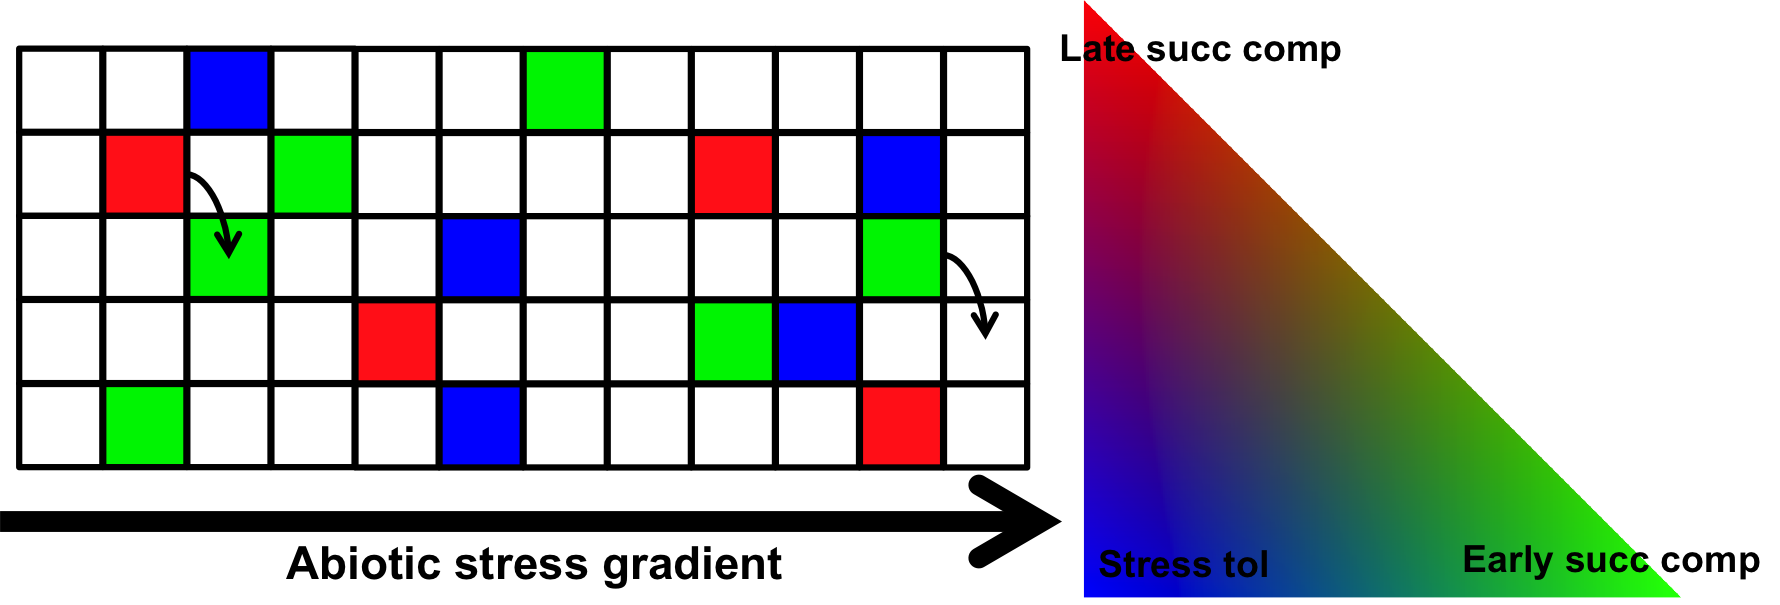
\includegraphics{../figures/auto.png}
\caption{\textbf{Cellular cellular automaton representing species
    dynamics along a rectangular landscape set along an abiotic
    gradient. Each cell is occupied by only one individual and
    dispersion is within the 8 neighboring cells. Species are
    defined by three traits defining a triangular tradeoff
    between early- or late-successional competitive ability
    \textit{vs.} climate stress tolerance.} 
\label{fig:triangtrade}}
\end{figure}

\subsection{Results}

\begin{figure}[ht]
\centering
\includegraphics{../figures/map_theo_K100.pdf}
\caption{\textbf{Simulation of species distribution along a abiotic stress gradient.}
\label{fig:mapK100}}
\end{figure}


\clearpage


\bibliographystyle{amnat}
\bibliography{references}
\end{document}

%%  LocalWords:  LMA WD optimisation Falster successional LLS et
%%  LocalWords:  Glopnet stomatal Farquhar Poorter RGR Charrier
%%  LocalWords:  cavitation cavitated Skelton Isohydric Onoda al
%%  LocalWords:  anisohydric Niinemets Simova Laughlin Fortunel
%%  LocalWords:  Douma VanBodegom Kooyman rainforests
